\documentclass{article}

\usepackage{amsthm}
\usepackage{amsmath}
\usepackage{amsfonts}
\usepackage[margin=1in]{geometry}
\usepackage{hyperref}
\usepackage{tikz}

\DeclareMathOperator{\im}{im}
\DeclareMathOperator{\re}{re}
\DeclareMathOperator{\len}{len}
\DeclareMathOperator{\res}{res}

\renewcommand{\epsilon}{\varepsilon}

\title{\href{https://math.umn.edu/sites/math.umn.edu/files/exams/complexf19.pdf}{Fall 2019 Complex Analysis Preliminary Exam}}
\author{University of Minnesota}
\date{}
\begin{document}
\maketitle

Where possible, computations have been also done using SageMath code available on GitHub at \\ github.com/tekaysquared/prelims (feel free to make pull requests!)

\begin{enumerate}
	\item Give a conformal mapping from the (open) upper half-disk $H = \{z : |z|<1 \text{ and } \im(z) > 0\}$ to the slit disk
	\[D = \{ z \in \mathbb{C} : |z|< 1,\;z \not \in [0,1] \]
	
	\begin{proof}
		First, let $f(z) = 1/z$. Then $f(H) = \{ z : |z|>1 \text{ and } \im(z) > 0 \}$. Since both $f$ and $f^\prime(z) = -z^{-2}$ are never $0$, 
		$f$ is a conformal mapping.
		%
		Now let $g(z) = z^2$. Then $g(f(H)) = \{ re^{i \theta} : r > 1 \text{ and } \theta \in (0, 2\pi) \}$. 
		$g=0$ and $g^\prime = 0$ only at $z = 0$, which is not in $f(H)$ so $g \circ f$ is a conformal mapping from $H$ to $g(f(H))$.
		%
		Finally, note that $f \circ g \circ f(H) = D$. 
		Again $f^\prime$ is never zero so the composition $f \circ g \circ f : H \rightarrow D$ is a conformal mapping.
	\end{proof}

	\setcounter{enumi}{1}
	
	\item Write the first three terms of the Laurent expansion of $\displaystyle f(z) = \frac{1}{z(z-1)(z-2)}$ centered at $0$ and convergent in $|1| < z < |2|$
	
	\begin{proof}
		The core idea of the computation is to split the function into a product of power series.
		First, we observe that 
		\[ \frac{1}{z-1} = \frac{1}{z(1-1/z)}\] 
		and see the geometric series 
		\[ \frac{1}{1-1/z} = \sum_{n=0}^\infty \left( \frac{1}{z} \right)^n,\]
		which converges for $|1/z| < 1$, or equivalently $|z|>1$.
		Similarly we see that 
		\[ \frac{1}{z-2} = \frac{-1}{2(1-z/2)} = -\frac{1}{2} \sum_{n=0}^\infty \left ( \frac{z}{2} \right )^n \]
		for $|z/2| < 1$, which is to say for $|z|< 2$.
		Thus we have
		\begin{align*}
			f(z) &= \frac{1}{z} \left ( \frac{1}{z} \sum_{n=0}^\infty \left ( \frac{1}{z} \right )^n \right ) \left ( \frac{-1}{2} \sum_{n=0}^\infty \left( \frac{z}{2} \right)^n \right )\\
			&= \frac{-1}{2z} \left (\frac{1}{z} + \frac{1}{z^2} + \frac{1}{z^3} + \cdots  \right) \left ( 1 + \frac{z}{2}+\frac{z^2}{4}+\frac{z^3}{8}+\cdots \right ).
		\end{align*}
		Note that the above product converges when each term converges, which is to say on the annulus $1 < |z| < 2$.
	
		Now note that the coefficient of 	$z^{-1}$ of the Laurent expansion is 
		\begin{align*}
			- \frac{1}{2} \left ( \frac{1}{2} + \frac{1}{4} +\frac{1}{8} + \cdots \right ) &=  \frac{-1}{2} \left [ \sum_{n \geq 0} (1/2)^n - 1\right ] \\
			&= -\frac{1}{2} \left (\frac{1}{1-1/2} - 1 \right)\\
			&= -\frac{1}{2}.
		\end{align*}
		
		The coefficient of $z^{0}$ is 
		\begin{align*}
			-\frac{1}{2} \left ( \frac{1}{4} + \frac{1}{8} + \frac{1}{16} +\cdots \right ) 
			&= -\frac{1}{2} \left(2 - 1 - \frac{1}{2}\right) = -1/4 \\
		\end{align*} 
		
		The coefficient of $z^1$ is
		\begin{align*}
			-\frac{1}{2} \left ( \frac{1}{8} + \frac{1}{16} + \frac{1}{32} + \cdots \right ) &= - \frac{1}{2} \left ( 2 - 1 - \frac{1}{2} - \frac{1}{4} \right )\\
			&= - \frac{1}{8}.
		\end{align*}
		 
		Therefore \[ f(z) = \cdots - \frac{1}{2z} - \frac{1}{4} - \frac{z}{8} + \cdots \]
	\end{proof}
	
Note that there is also a Laurent series which converges for the annulus $0 < |z| < 1$. This can be found by using the geometric series expansion \[\frac{1}{z-1} = \frac{-1}{1-z} = - \sum_{n=0}^\infty z^n\] which of course converges for $|z|< 1$, and using the same expansion of $\frac{1}{z-2}$ as above. This is the one provided by SageMath. For another example of this, see \href{https://math.stackexchange.com/questions/2553132/laurent-series-for-different-domains}{this math StackExchange post}.

	\item Classify entire functions $f$ so that $|f(z)| \leq C |z|$ for some constant $C$.
	
	\begin{proof}
		Liouville's theorem tells us that bounded, entire functions are constant. 
		%
		If $f(z)/z$ is entire, then Liouville's theorem would tell us that $f(z)/z$ is a constant (call it $k$), and so since $f(z)/z = k$, then $f(z) = kz$.
		%
		If $f(z)/z$ is not entire, then there is a simple pole at $z=0$ (since $f(z)$ is entire). 
		This would imply that in (e.g.) the open disk centered at $z_0 = 1$ with radius $1$, we would have $f(z)/z$ being unbounded. 
		But this contradicts that $|f(z)/z| \leq C$ is bounded on all of $\mathbb{C} - \{0\}$.
		
		Thus, the functions $f$ which satisfy $|f(z)| \leq C |z|$ are linear functions with no constant term.
	\end{proof}

	\newpage
	\item Evaluate $\displaystyle \int_{-\infty}^\infty \frac{\cos(x)}{1+x^2} dx$. 
	% WolframAlpha tells us the answer is pi/e 
	% See residue theorem and estimation lemma on Wikipedia 
	
	\begin{proof}
		
		
		We compute this real integral by passing to complex values and computing.
		
		Define \[f(z) = \frac{e^{iz}}{1+z^2} = \frac{e^{iz}}{(z+i)(z-i)}.\] 
		We make this choice of $f$ because for $x$ on the real axis, we have $f(x) = \frac{\cos(x) + i \sin(x)}{1+x^2}$, which is to say
		$\re f(x) = \frac{\cos (x)}{1+x^2}.$ 
		
		
%		But since $\cos$ is an even function $\cos (-x) = \cos x$ thus \[\re f(x) = \frac{\cos (x)}{1+x^2}\] which is the integrand of the integral which we are trying to compute.
%		We will thus compute  \[\re \left(\int_{-\infty}^\infty f(z) dz \right) = \int_{-\infty}^\infty \frac{\cos(x)}{1+x^2} dx\]
%		
		For $t > 1$, let $\gamma_t$ denote the union of the line from $[-t,t]$ with the semi-circle of radius $t$ in the upper half-plane (call it $C_t$), with the orientation of $\gamma_t$ being counter clockwise.
		
		Visually:
		
		\begin{center}
		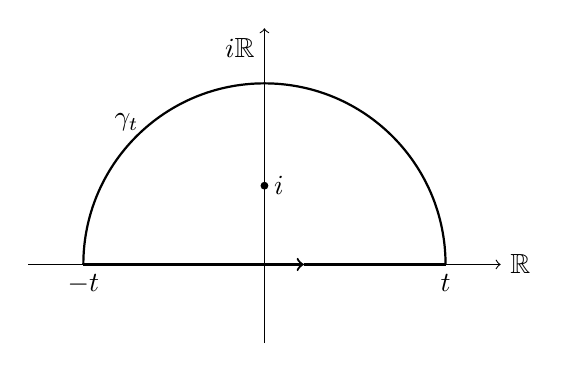
\begin{tikzpicture}
			%\draw[step=1cm,gray,very thin] (-2.9,-0.9) grid (2.9,2.9);
			\draw[thin,->] (0,-1) -- (0,3); 
			\draw[thin,->] (-3,0) -- (3,0);
			
			\node[anchor = north east] at (0,3) {$i \mathbb{R}$};
			\node[anchor = west] at (3,0) {$ \mathbb{R}$};
			
			\node[fill = black, inner sep=1pt, circle] at (0,1) {};
			\node[anchor = west] at (0,1) {$i$};
			
			\node[anchor = north] at (2.3,0) {$t$};
			\node[anchor = north] at (-2.3,0) {$-t$};
			
			\node at (-1.75,1.8) {$\gamma_t$};
			
			\draw[thick] (2.3,0) arc (0:180:2.3) ;
			\draw[thick,->] (-2.3,0) -- (0.5,0) ; 
			\draw[thick] (0.5,0)--(2.3,0);
		\end{tikzpicture}
		\end{center}
		
		By the residue theorem, we know that as long as $t > 1$ 
		\[ \int_{\gamma_t} f(z)dz = 2\pi i \res_{i} f(z) .\]
		
		Since $i$ is a simple pole of $f(z)$ (as seen by the factorization $1+z^2 = (z+i)(z-i)$), we can compute 
		\begin{align*}
			\res_i f &= \lim_{z \rightarrow i} (z-i) f(z)\\
			&= \lim_{z \rightarrow i} (z-i)\frac{e^{iz}}{(z+i)(z-i)}\\
			&= \lim_{z \rightarrow i}\frac{e^{iz}}{(z+i)} \\
			&= \frac{e^{-1}}{2i} = \frac{1}{2ie}
		\end{align*}
		and so 
		\[ \int_{\gamma_t} f(z)dz = 2\pi i\frac{1}{2ie} = \frac{\pi}{e}  .\]
		
		We can split up the integral of $f(z)$ over $\gamma_t$ along the real axis and the semi-circle as
		\[\int_{\gamma_t} f(z) dz = \int_{[-t,t]} f(z) dz + \int_{C_t} f(z) dz.\]
		
		The estimation lemma or ``ML inequality" tells us that since the length of a semicircle of radius $r$ is $\pi r$, then
		\begin{align*}
			\left | \int_{C_t} f(z) dz  \right | &\leq \pi t \max_{z \in C_t} |f(z)|
		\end{align*}
		
		We now compute an upper bound for $ \max_{z \in C_t} |f(z)|$, 
		\begin{align*}
			\left | \frac{e^{iz}}{1+z^2}\right | = \frac{ | e^{iz} | }{|1+z^2|}
		\end{align*}
		
		Note that $C_t$ only contains points with $\im z > 0$, and so if $z = x + i y$, then 
		${|e^{iz}| = |e^{ix - y}| = e^{-y} < 1}$
		thus in $C_t$
		\[\left | \frac{e^{iz}}{1+z^2}\right | \leq \frac{ 1 }{|1+z^2|}\]
		
		The reverse triangle inequality tells us (again only considering $z \in C_t$) that \[|z^2 - (-1) | > \left ||z^2| - | -1|\right| = \left ||z|^2 - 1\right| = |t^2 - 1|\]
		And so
		thus in $C_t$
		\[\left | \frac{e^{iz}}{1+z^2}\right | \leq \frac{ 1 }{|t^2-1|}\]. 
		
		Taking the limit as $t \rightarrow \infty$ we see that the integral over $C_t$ goes to zero, and so
		
		\[ \lim_{t \rightarrow \infty } \int_{\gamma_t} f(z)dz =  \lim_{t \rightarrow \infty} \int_{[-t,t]} f(z) dz = \int_{(-\infty, \infty)} f(z) dz .\]
		
		But the integral over $\gamma_t$ is independent of $t$, and so
		\[\int_{(-\infty, \infty)} f(z) dz = \pi/e.\]
		
		Recall that the integral we \textit{wanted} to compute was the real part of the above integral, but since the integral is real, the real part is the whole integral, and so
		
		\[\int_{-\infty}^\infty \frac{\cos x}{1+x^2} dx = \frac{\pi}{e}\]
		
	\end{proof}
	
	
	\item Determine the radius of convergence of the power series for $z \log z$ at $z_0 = -3 + 4i$.
	
	\begin{proof}
		We will look for the largest $R$ for which there is a disk $D_R$ of radius $R$ centered at $z_0$ on which there is a holomorphic function agreeing with $z \log z$.
		%
		The product of holomorphic functions is holomorphic, so because $g(z) = z$ is entire, the radius of convergence of $z \log z$ is limited by $f(z) = \log z$. 
		
		To find the radius of convergence of $f$ at $z_0$, observe that there is no number $w \in \mathbb{C}$ such that $e^w = 0$, and so the $R$ is bounded above by $|-3 + 4i - 0| = 5$.		
		
		On the other hand recall that it is a theorem\footnote{Theorem 6.1 in Chapter 3 of Stein and Shakarchi's \textit{Complex Analysis}} that if $D$ is a simply connected region which does not contain $0$, then there is a branch of the logarithm (call it $\log_D$) which is holomorphic on $D$. Consider the (open) disk $D_5$ of radius 5 centered at $z_0$. Clearly this does not contain $0$, and so there is a holomorphic $\log_{D_5}$. Thus, we see $R \geq 5$. 
		
		Since $R \leq 5$ and $R \geq 5$, we have $R = 5$.
	\end{proof}
	

	\item Let $f,g$ be holomorphic functions on $\{z : |z| < 2\}$ with $f$ nonvanishing on $|z| = 1$. Show that for all sufficiently small $\epsilon>0$ the function $f+ \epsilon g$ has the same number of zeros inside $|z| = 1$ as does $f$. 
	
	\begin{proof}
		Since $f,g$ are holomorphic on $\{ z: |z| < 2\}$, they are holomorphic on the compact sets $D = \{z : |z | \leq 1\}$ and its boundary $\partial D =\{z : |z| = 1\}$.
		
		Rouche's theorem states that if $|\epsilon g| \leq |f|$ on $\partial D$ (which can be thought of as a closed curve) then $f$ and $f+ \epsilon g$ have the same number of zeros inside $D$. 
		Thus our goal will be to find $\epsilon > 0$ which establishes this bound.
		
		Since $f,g$ are holomorphic on $\partial D$, they are continuous, and since $\partial D$ is a closed subset of $\mathbb{C}$, it is compact.
		The modulus function is also continuous, and so by composition,		
		$|f|,|g|$ are both continuous real-valued functions and thus achieve a maximum and minimum on $\partial D$.
		
		Let $m = \min_{z \in \partial D} f$ and $M = \max_{z \in \partial D} g$. Pick $\epsilon < \frac{m}{M}$. Then on $\partial D$ 
		\begin{align*}
			| \epsilon g | &= \epsilon |g|\\
			& < \frac{m}{M} |g|\\
			& \leq \frac{m}{M}M\\
			&= m \leq |f|.
		\end{align*}
	\end{proof}

%	\item Show that the curve $z^2 + w^2 = 1$ has genus $0$.
%	
%	This is a hyper elliptic curve since $z^2 = 1-w^2$.
	
\end{enumerate}

\end{document}